\documentclass{sigchi}

% Use this command to override the default ACM copyright statement (e.g. for preprints). 
% Consult the conference website for the camera-ready copyright statement.


%% EXAMPLE BEGIN -- HOW TO OVERRIDE THE DEFAULT COPYRIGHT STRIP -- (July 22, 2013 - Paul Baumann)
% \toappear{Permission to make digital or hard copies of all or part of this work for personal or classroom use is  granted without fee provided that copies are not made or distributed for profit or commercial advantage and that copies bear this notice and the full citation on the first page. Copyrights for components of this work owned by others than ACM must be honored. Abstracting with credit is permitted. To copy otherwise, or republish, to post on servers or to redistribute to lists, requires prior specific permission and/or a fee. Request permissions from permissions@acm.org. \\
% {\emph{CHI'14}}, April 26--May 1, 2014, Toronto, Canada. \\
% Copyright \copyright~2014 ACM ISBN/14/04...\$15.00. \\
% DOI string from ACM form confirmation}
%% EXAMPLE END -- HOW TO OVERRIDE THE DEFAULT COPYRIGHT STRIP -- (July 22, 2013 - Paul Baumann)


% Arabic page numbers for submission. 
% Remove this line to eliminate page numbers for the camera ready copy
% \pagenumbering{arabic}


% Load basic packages
\usepackage{balance}  % to better equalize the last page
\usepackage{graphics} % for EPS, load graphicx instead
\usepackage{times}    % comment if you want LaTeX's default font
\usepackage{url}      % llt: nicely formatted URLs
\usepackage{siunitx}
\usepackage{cite}
\usepackage{dblfloatfix}

% llt: Define a global style for URLs, rather that the default one
\makeatletter
\def\url@leostyle{%
  \@ifundefined{selectfont}{\def\UrlFont{\sf}}{\def\UrlFont{\small\bf\ttfamily}}}
\makeatother
\urlstyle{leo}


% To make various LaTeX processors do the right thing with page size.
\def\pprw{8.5in}
\def\pprh{11in}
\special{papersize=\pprw,\pprh}
\setlength{\paperwidth}{\pprw}
\setlength{\paperheight}{\pprh}
\setlength{\pdfpagewidth}{\pprw}
\setlength{\pdfpageheight}{\pprh}

% Make sure hyperref comes last of your loaded packages, 
% to give it a fighting chance of not being over-written, 
% since its job is to redefine many LaTeX commands.
\usepackage[pdftex]{hyperref}
\hypersetup{
pdftitle={Skintillates: Towards Epidermal Interactions},
pdfauthor={LaTeX},
pdfkeywords={SIGCHI, proceedings, archival format},
bookmarksnumbered,
pdfstartview={FitH},
colorlinks,
citecolor=black,
filecolor=black,
linkcolor=black,
urlcolor=black,
breaklinks=true,
}

% create a shortcut to typeset table headings
\newcommand\tabhead[1]{\small\textbf{#1}}
\newcommand{\ignore}[1]{}

%stop hyphenation
\tolerance = 1
\emergencystretch = \maxdimen

% End of preamble. Here it comes the document.
\begin{document}

\title{Skintillates: Towards Epidermal Interactions}

\numberofauthors{3}
\author{
  \alignauthor 1st Author Name\\
    \affaddr{Affiliation}\\
    \affaddr{Address}\\
    \email{e-mail address}\\
    \affaddr{Optional phone number}
  \alignauthor 2nd Author Name\\
    \affaddr{Affiliation}\\
    \affaddr{Address}\\
    \email{e-mail address}\\
    \affaddr{Optional phone number}    
  \alignauthor 3rd Author Name\\
    \affaddr{Affiliation}\\
    \affaddr{Address}\\
    \email{e-mail address}\\
    \affaddr{Optional phone number}
}

\maketitle

\begin{abstract}
Skintillates is a wearable technology that mimics tattoos - the oldest and most commonly used on-skin displays in human culture. We demonstrate that by fabricating electrical traces and thin electronics on temporary tattoo paper, a wide array of displays and sensors can be created. Just like the traditional temporary tattoos often worn by children and adults alike, Skintillates flex naturally with the user’s skin. Our simple fabrication technique also enables users to freely design and print with a full range of colors to create application-specific customized designs. We demonstrate the technical capabilities of Skintillates as sensors and as expressive personal and private displays through a series of application examples. Finally, we detail the results of a set of user studies that highlight the user experience, comfort, durability, acceptability, and application potential for Skintillates. 
\end{abstract}

\keywords{
  Fabrications; wearable; skin; epidermis; tattoo  \newline
}

\category{H.5.m.}{Information Interfaces and Presentation (e.g. HCI)}{Miscellaneous}

\section{Introduction}
\begin{figure}[!h]
\centering
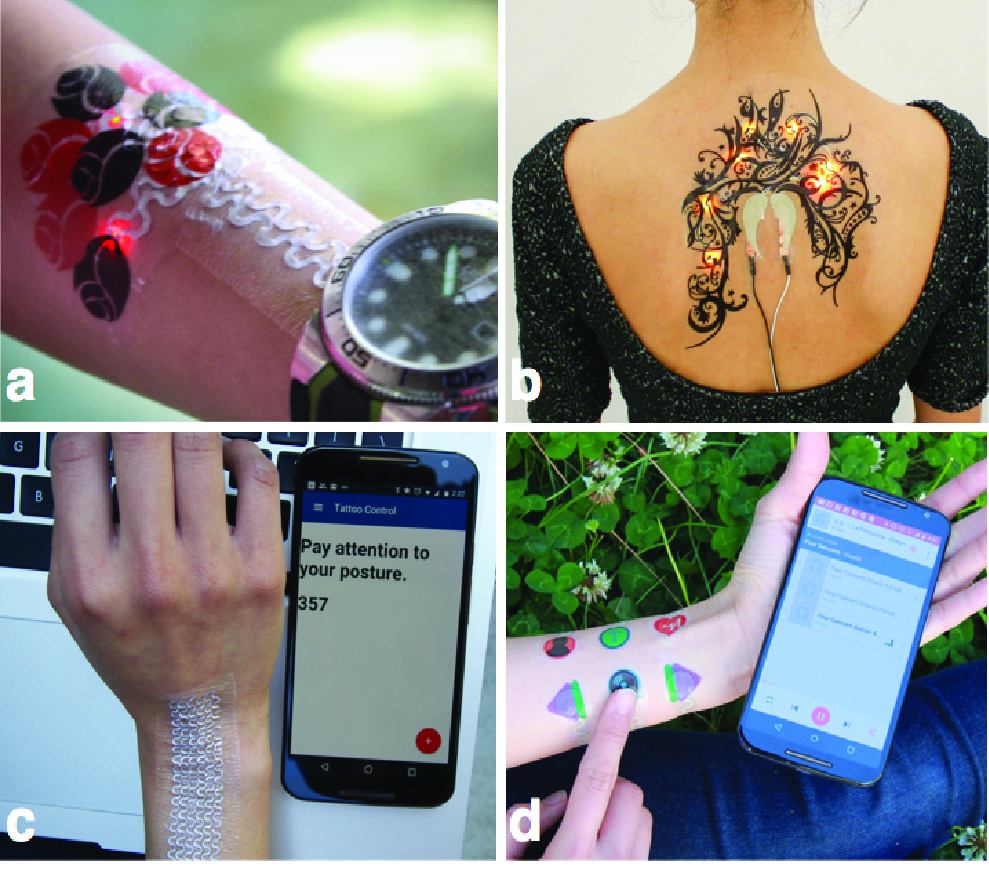
\includegraphics[width=1\columnwidth]{figures/Figure1}
\caption{Skintillates is a class of temporary tattoo electronics that can be fabricated using an accessible process. a) A point-light display, b) A back tattoo LED display that flashes with music, c) A strain gauge that detects body position, d) capacitive buttons for mobile device control}
\vspace{-8pt}
\label{fig:overall}
\end{figure}
Every day, we interact with the world through our skin. The human skin senses important events that happen closest to us, and serves as an expressive medium when adorned with tattoo art. In this paper, we present Skintillates, a class of novel epidermal wearable interactive devices. Skintillate devices can serve as passive and active on-skin displays, capacitive and resistive sensors for electronic device control, and strain gauges for posture detection. The combined thickness of the substrate and traces of Skintillates is thinner than a human hair - approximately 36\SI{}{\micro\metre}. The devices move naturally with the user’s skin and are comfortable to wear for long periods of time. Similar to traditional tattoos, Skintillates can be customized to be a variety of different shapes and colors to fit the user's intended functions. Moreover, Skintillates are fabricated using an accessible, low-cost process that uses common commercially-available     materials     and      easy-to-obtain equipment. 

Skintillates is inspired by a line of research in micron-thin epidermal electronics pioneered by material scientists. Since these epidermal electronics directly contact the skin, they can be made into extremely accurate, yet comfortable, sensors. However, due to their intricate fabrication method, epidermal sensors to date remain to be a device mainly used in specialized medical and military applications. Responding to a clear need for ultra thin on-skin wearable electronics to enable natural and always-available interactions with the electronics and data around us\cite{MunehikoSato:2012we,chris:2011ve,ChrisHarrison:2010vi,DavidKim:2012uu,Harrison:2014ft,Laput:2014du}, we created Skintillates. Skintillates are a class of devices tailored for applications that focus more on everyday-interactions, and have a fabrication method much more open to experimentation for sophisticated visual and electrical design. To list a few examples, Skintillates can serve as programmable LED displays with customized aesthetic design(Fig.\ref{fig:overall}a-b), strain gauges that respond to body movement (Fig.\ref{fig:overall}c)), and capacitive sensors for mobile device control with visual designs that indicate the applications they affect (Fig.\ref{fig:overall}d). 

\section{Motivation}
Skintillates aims to enable a new form of interaction and expression through electronically-augmented temporary tattoos that can be easily designed and fabricated, and comfortably worn. Beyond the technical design of our system, we surveyed the historical, cultural, and deeply personal embedded meaning of tattoos and body art to further refine what Skintillates should be.

\subsection{Towards Technological Tattoos: A Brief Cultural History}

Tattoos are known to have been part of human culture from as far back as the 4th millennium BC and used as forms of religious,  tribal, and personal  identification  and adornment \cite{Grognard:o1z3U5M2}. In today's culture, expressing  one's  love  for the combination of technology and arts through body-modifications varies in degrees from  embedding  ferrous  materials  under one’s skin \cite{Norton:OK5Z52w0}, to tattooing math equations and the molecular structure of plants onto one's body \cite{Zimmer:2011wb}. 

With the increasing popularity of using temporary tattoos as a platform for artistic self-expression\cite{Fanning:v_9LfC8A,ByCourtneyRubin:tj}, it is evident that the cultural role of the skin as a canvas for personal expression is still as relevant today as it has been in the past, but in some cases with a bit less permanence.  This, combined with the desire to incorporate technology with the arts, would seem to point to a need for wearable devices that are in and of themselves an expression of one's self, culture, or beliefs, while being safe and interchangeable to match the interest of the day. Skintillates explores how visual body elements can become more interactive and expressive by capturing part of the allure of the rich tattoo culture. 

Since the beginning of the tattoo culture, wearers of tattoos, both permanent and temporary ones, expect control of the aesthetic of the tattoos because body art sends a strong message about the wearer\cite{Doss:2009ee,McLeod:2014ua}. To that end, Skintillates specifically allows the customization of the visual aesthetic and the electronic functionally, enabling open, creative, and personal designs in an on-skin wearable device.

\subsection{Public and Private by Design}
Diane Ackerman wrote in \textit{A Natural History of the Senses}, ``Tattoos make unique the surface of one's self, embody one's secret dreams, adorn with magic emblems the Altamira of the flesh\cite{Mifflin:2013ux}.''Tattoos can serve a dual role as both a narrative to the public and as a private message to the wearer \cite{Doss:2009ee,McLeod:2014ua}. We foregrounded the flexibility and hybridity of the shifting public and private tensions in one of our sample applications of Skintillates. Skintillates also affords a wide range of personal designs varying in size, shape, color, body location, sensing, and electronic properties. We demonstrate and study examples of how the customization of Skintillates can allow these wearable devices to serve as both public and private displays in this paper. 

\subsection{Comfort, Safety, and Biocompatibility}
Any wearable, from clothing to electronics to tattoos, must be safe and comfortable to wear for long periods.  Skintillates uses materials for the substrate and traces that have been approved by U.S. Food and Drug Administration (FDA) for safe usage human skin. To minimize the possibility of negative skin-reaction to Skintillates, we used commercially available temporary tattoo paper as the substrate, and a medical electrode grade silver screen-printing ink as the conductive material for the circuitry\cite{Anonymous:6vWXbuD5,Cristea:2009uq,Rattfalt:2013ts}. In some Skintillate devices where electronic parts such as ICs and LEDs are used, the current is limited to 10mA, which is considered physiologically safe for humans \cite{Scherz:_BfVY1Mg}. 
%In one of the application examples, standard surface mount electronic parts are used. While most IC are made with inert materials that interact with skin, we hope to perform more studies or 

\section{Related Work}
Skintillates builds off of a body of related work across Human-Computer Interaction (HCI), flexible polymers, and Epidermal Electronics as we detail below.
\subsection{On-Body Interfaces}
Our own body is our most intimate and familiar interactive device. Technological advancements in fields such as optics, materials sciences, and signal acquisition and processing, have enabled HCI researchers to imagine and create sensors and controls directly on the user’s skin. Many of these projects aim to create an always-on, unobtrusive, responsive technology that allows users to interact in natural and intuitive ways with their personal devices and environment. Optical projection and careful image processing transforms the user’s skin into an interactive display  screen  in  work  such   as   Skinput   and Skinbuttons \cite{ChrisHarrison:2010vi, Laput:2014du}. Saponas and his colleagues obtained Electromyography (EMG) from users’ forearms to create a natural and always-available computer interface \cite{Anonymous:2009ua}. To explore creative input methods in addition to vibration and visual, Ion led an effort that created a skin drag display that communicated messages to the user by drawing  on their skin with a ``tactor'' \cite{Ion:2015ig}. Other researchers imagined an implanted device as an always-available intimate input and output \cite{Holz:2012ti}. We designed Skintillates from the inspirations offered by these and similar HCI work in on-body interaction.

\subsection{Polymeric On-skin Wearables}
The flexibility of polymer makes it a great substrate for wearable electronics. Great advances have been made in many applications, including robotic skin that can detect the touch of a fly via capacitive sensing\cite{Mannsfeld:2010is}, fully-functional on-skin keypads\cite{Anonymous:L82kTfjJ}, highly-stretchable strain gauge-based wearable interfaces \cite{Boley:2014dr,Muth:2014bv}, ultra-flexible sensing circuits that include radio capability\cite{Jang:1gb,Anonymous:BBKIC9BZ}, and adaptive camouflage skin overlay\cite{Yu:2014ht}. The thickness and relatively high tensile modulus of polymeric wearable devices makes them durable and highly reusable, providing the ideal substrate for encapsulating complex electronics.

However, the same properties that make polymeric wearables functional and reusable also often make them uncomfortable to wear for long periods since they are typically not very breathable on-skin without special device design \cite{Jang:1gb}. Moreover, to fabricate polymeric substrates that are uniformly thin for on-skin wearable applications, specialized and expensive equipment such as a spinner and vacuum chamber are often needed \cite{Son:2014iya,Yu:2014ht,Anonymous:BBKIC9BZ,Jang:1gb,Muth:2014bv,Anonymous:L82kTfjJ}. 

Additionally, the creation of a flexible conductive polymeric material is non-trivial.  Typically, this is accomplished through the mixing of conductive materials with nonconductive polymer or by injecting liquid metal into prefabricated channels. On the one hand, mixing a conductive material, such as graphite, into a nonconductive polymeric carrier is a simple process, but the resulting conductivity tends  to  be  extremely poor\cite{Weigel:2015fh,Frutiger:2015fm}. On the other end of the spectrum, better electrically performing materials such as highly conductive liquid  metal  are unsuitable for on-skin applications due to their extreme toxicity \cite{Boley:2014dr}. 

These material limitations often make customizing the visual appearance of polymeric wearables difficult as well. One such example of a polymeric wearable device using this technique is iSkin\cite{Weigel:2015fh}, which addressed these problems by cutting the black graphite-functionalized conductive polymer into visually attractive patterns, thus cleverly turning the electrical layer into an aesthetically customizable layer. Skintillates seeks to expand on this work by broadening the visual design freedom by moving from purely monochromic art to a full range of inkjet printable colors, as well as developing techniques that can produce a thinner, more comfortable on-skin interface that supports additional input/output modalities. 

%The limitation of this technique lies in the lack of control over the color of the conductive polymer, thus reducing the visual design freedom of the wearable devices.


\subsection{Epidermal Electronics}
Human skin has natural wrinkles, creases, and pits that are on the order of \SI{15}{\micro\metre} to \SI{100}{\micro\metre}\cite{Tchvialeva:2014wla}. If the wearable electronics have a thickness smaller than or comparable to natural skin feature sizes, the wearer will not feel his/her skin unnaturally restrained\cite{Kim:2011bv}. Recent approaches have worked to address these epidermal surface and scale issues. The “Epidermal Electronics”, as defined by Kim et al, refers to the class of sensors with thickness on the order of natural skin creases, conforms to small skin movements such as wrinkling, and presents minimal obstructions to user's skin sensations \cite{Kim:2011bv}. Multifunction electronics, such as capacitive sensors that accurately detect noisy physiological signals, multilayer coils that enable on-skin RF communications, and strain and hydration sensors that aid in post-operation recovery\cite{Jeong:2013km,Kim:2014iq,Bandodkar:2014dl,Kim:2011bv} are possible with these ultra-thin devices. Materials that are structurally stronger, such as polymeric stamps, water-soluble Poly(vinyl alcohol) (PVA), or skin-safe stickers are used as a structural backing to transfer the ultra-thin Epidermal Electronic devices onto the user's skin\cite{Son:2014iya}. Once transferred, the ultra-thin Epidermal electronics, with low Young's modulus that matches with human skin, can be attached to skin through van der Waals force alone without additional adhesive \cite{Son:2014iya,Kim:2011bv}. 

Despite the impressive scientific advances made by the development of Epidermal Electronics, their fabrication process makes them inaccessible to the general public. The flexibility and conformity of epidermal electronics enabled by the ultra-thin geometry comes at the expense of a complicated fabrication methods and equipment, such as a photoresist spinner, e-beam evaporator, mask aligner, and chemical etch bay\cite{Kim:2011bv}. The fine electrical traces (down to \SI{1}{\micro\metre} in width), and the ultra-thin conductive and insulation layers (ranges from 500nm to 5\SI{}{\micro\metre}), though extremely sensitive and conformal to the human skin, require highly specialized lithographic equipment, high temperature metal deposition, and etching chemicals to fabricate\cite{Kim:2011bv,Kim:2014iq}. In one example application of Epidermal Electronics, a small piece of temporary tattoo paper is used as a backing to transfer the epidermal device onto the user's skin\cite{Kim:2011bv}. Unfortunately, the etching process that fabricates the fine gold traces is incompatible with commercially available tattoo paper because the paper cannot withstand the chemical etchants. Skintillates overcomes this barrier by replacing the cleanroom fabrication steps with a low-temperature screen-printing process. As a result, Skintillates enables users to customize the device both electronically and aesthetically.  More importantly, this makes Skintillates accessible to a broad range of users since they can be fabricated at a much lower cost without cleanroom equipment or extreme temperatures. 

\section{Systems Details and Fabrication}
 All Skintillates are comprised of five basic layers (Fig.\ref{fig:layers}). Three of these layers come as a commercially available package. Skintillates are fabricated on temporary tattoo paper, which rests on top of a paper backing before the tattoo is applied. A nonconductive inkjet-printed art layer can be printed on the tattoo substrate before the electrically functional conductive layer is screen-printed on top. Additional layers, such as an electronics layer, can be added to enable more complex interactions and expressivity. Before applying the Skintillate device onto a user's skin, an adhesion layer is applied on top of the Skintillates device. 

\begin{figure}[h]
\centering
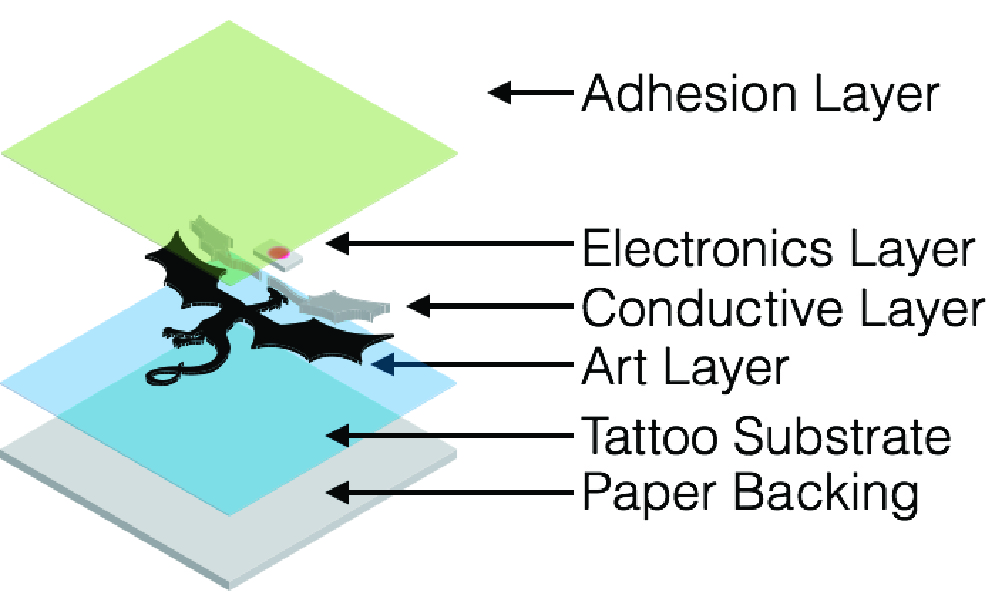
\includegraphics[width=0.9\columnwidth]{figures/Figure4}
\caption{An illustration of the different layers of a basic Skintillate device.}
\vspace{-8pt}
\label{fig:layers}
\end{figure}

\begin{figure*} [!ht]
\centering
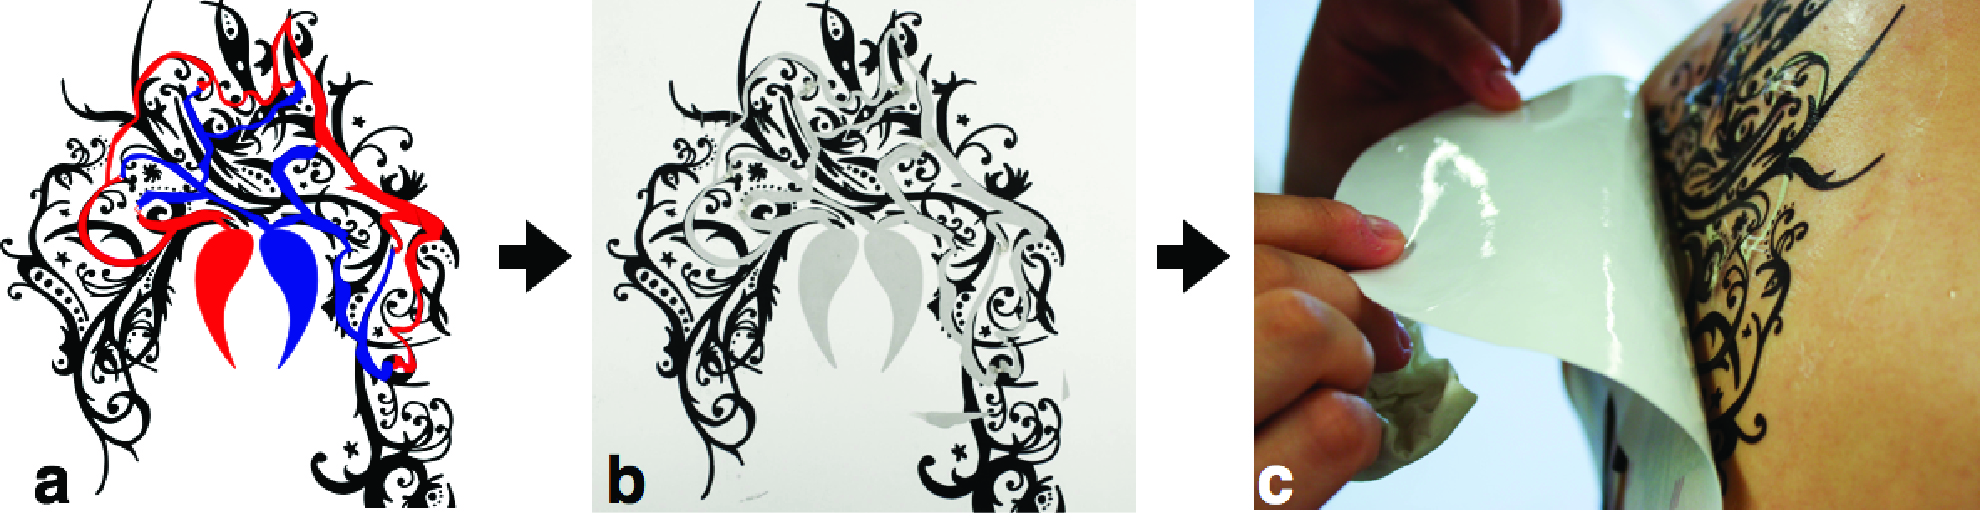
\includegraphics[width=1.0\textwidth]{figures/Figure3}
\caption{Skintillates fabrication process work flow. a) the art layer (in black) and the electrical traces (in red and blue) are designed in a standard design program, b) the art layer (in black) is inkjet printed and the conductive layer (in silver) screen-printed on the tattoo substrate, and c) the Skintillate device is applied on skin and released from  the paper backing.}
\vspace{-8pt}
\label{fig:applicationprocess}
\end{figure*}

 There were four major goals that guided our design when creating Skintillates:

\begin{itemize}
  \item \textbf{Functional}-provide electronics that are conductive enough to support body based HCI applications such as sensing and output displays
  \item \textbf{Comfortable}-fabricate with materials that are thin (ideally less than 100\SI{}{\micro\metre} to fit within natural wrinkles), skin conforming, unobtrusive, and can be comfortably worn for hours or days and then easily removed
  \item \textbf{Durable}-remain functional over typical usage of hours or days. 
  \item \textbf{Aesthetically Expressive}-the substrate has to be easily customizable to enable a broad range of  artistic expressions and user personalizations 
\end{itemize}

Similar to Epidermal Electronics, we aimed for the look and feel of electronic-integrated-with-skin aesthetic in Skintillates. We developed a fabrication process that relied on inexpensive equipment and materials, and we looked to the crafting community for some of our early inspiration. 

Screen-printing, which can be carried out with a relatively simple and inexpensive set of tools, was a great candidate for the Skintillates fabrication process. The screen-printing technique has been used to create work from beautiful arts and craft to fine and complicated flexible electronics by makers of all skill levels \cite{Olberding:2014ds,Perry:CXGigkdt,Dillon:2008uc}. We chose to directly screenprint circuits and sensors onto commercially available temporary tattoo papers. The silver screen-printable ink (\$100 for 25g) used was chosen because it is commonly used for fabricating medical devices and electrodes \cite{Cristea:2009uq,Rattfalt:2013ts}. Although we had successfully created these devices with both conductive inkjet printing and conductive pens, we decided against fabricating the Skintillates devices with them because of the lack of data in the safety and long-term biocompatibility of these inks. 

For the device substrate, we chose to use an inkjet-printable temporary tattoo paper (Silhouette Inkjet Printable tattoo paper, \$7.42 for four 8.5"x11" sheets). We believe temporary tattoo paper to be a good platform for Skintillates because 1) users can simply inkjet print the visual design of the tattoo directly onto the tattoo paper, and 2) as an existing product, their safety and comfort have already been well established. Moreover, temporary tattoos have an application process that is simple and well established. By building on top of a substrate that users are familiar with, we hope to enable Skintillates to be easily incorporated into user's everyday lifestyle.

\subsection{Fabrication and Application of Skintillates}
Skintillates are fabricated using a standard screen-printing process and are applied onto a user's skin the same way traditional temporary tattoos are applied. The full process of fabrication and application is detailed below.
\begin{enumerate}
  \item \textbf{Artwork Design}-Design artwork with any graphic design tool. (Black area of Fig.\ref{fig:applicationprocess}a)
  \item \textbf{Electronics Design}-Design the circuit and/or sensors (conductive layer) to be screen-printed as the conductive layer using the same design tool. (Blue and red area  of Fig.\ref{fig:applicationprocess}a) 
  \item \textbf{Print Art Design}-Use an inkjet printer to print the art layer design onto the tattoo substrate while it is still attached to its paper backing. 
  \item \textbf{Create Mask}-Cut a negative mask of the conductive layer with a vinyl cutter for screen-printing the conductive layer.
  \item \textbf{Attach Mask}-Apply vinyl mask onto the silkscreen.
  \item \textbf{Silkscreen Traces}-Screen-print the circuit and/or sensors using conductive silver screen-printing ink.(Fig.\ref{fig:applicationprocess}b) 
  \item \textbf{Populate Circuit}-Mount electronics onto the circuit using z-axis conductive tape at appropriate locations if needed. Apply copper tape or any desired connector to power the circuit. 
  \item \textbf{Prepare Skintillate Device for Application}-Apply the adhesive layer included in the temporary tattoo paper package.
  \item \textbf{Apply Tattoo}-Position the Skintillate device on the desired body location. Wet, press, and lift the paper backing (Fig.\ref{fig:applicationprocess}c) 
\end{enumerate}
Figure \ref{fig:micrograph} is a micrograph of a basic Skintillates device under magnification of 200x, which includes the tattoo substrate and a conductive layer, and is approximately 36\SI{}{\micro\metre} - thinner than an average human hair.  Most Skintillates are about the same size as this representation. Surface mount 0603 LEDs and resistors%ADD ARROWS POINTING TO OWL EYES TO SHOW THE LEDS
, which have thickness of  \SI{500}{\micro\metre}, were used throughout this study to minimize the added thickness in locations where they were mounted (Fig.\ref{fig:LED0603}). Increased complexity in electrical functionality and aesthetic design could be achieved by using extensions to this basic fabrication method. Some specific extensions will be discussed in the application section. 

\subsection{Cost and Fabrication Time}
We performed a cost and time analysis of fabricating a Skintillates device with some integrated electronics that wrap around the arm (Fig.\ref{fig:LED0603}). A Skintillates tattoo that measures 6.5 in x 1.0 in would cost \$0.23 in temporary tattoo paper and adhesive. It would take approximately 0.3g of silver screen-printing ink to fabricate the circuit, which would cost \$1.2. With \$0.5 allocated for two surface mount LEDs, the total cost of such a device is \$1.83. Such a tattoo would take less than 15 minutes to fabricate. The cost of any specific Skintillates device will vary with the design. For example, a large Skintillates device with many electrical silver traces will cost more than the aforementioned example device.  

\begin{figure}[!ht]
\centering
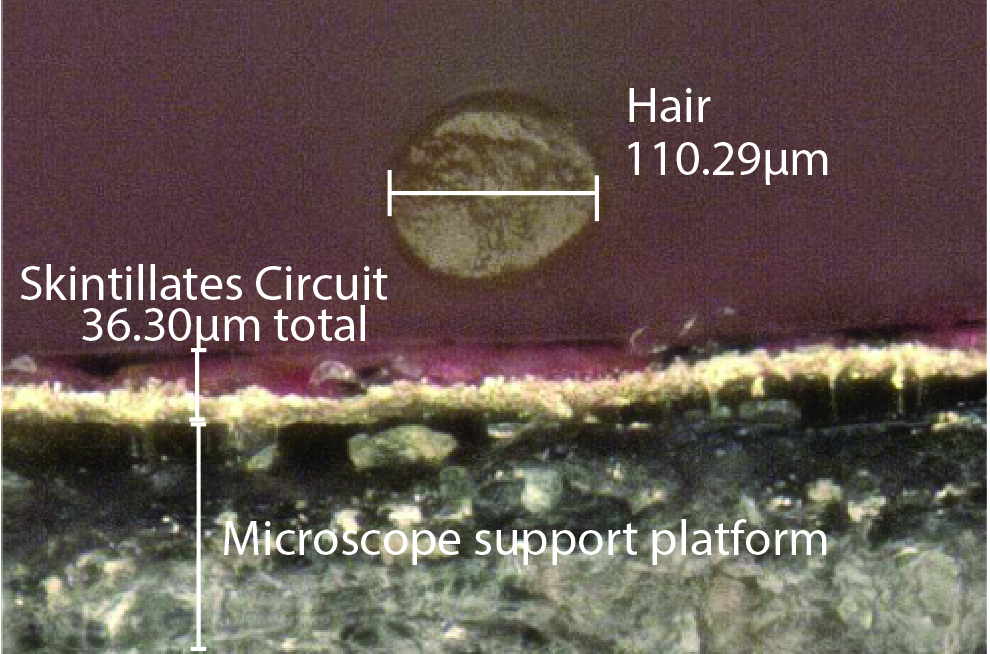
\includegraphics[width=1\columnwidth]{figures/Figure2}
\caption{A micrograph of the cross section of a \SI{36}{\micro\metre}-thick Skintillates device compared to a cross section of a human hair (\SI{110}{\micro\metre}).}
\vspace{-8pt}
\label{fig:micrograph}
\end{figure}

\begin{figure}
\centering
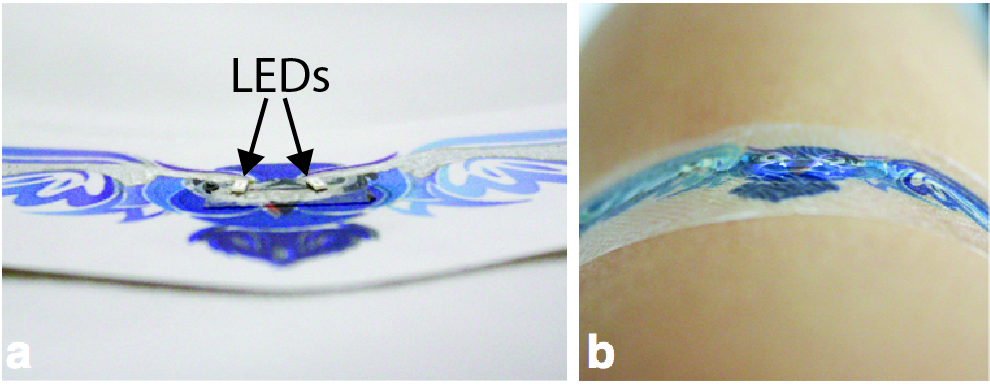
\includegraphics[width=1\columnwidth]{figures/LED0603}
\caption{A side view picture of Skintillates device, showing its conformal profile. a) A Skintillates device with 0603 LED. b) The same device worn on skin}
\vspace{-8pt}
\label{fig:LED0603}
\end{figure}

\begin{figure}[!h]
\centering
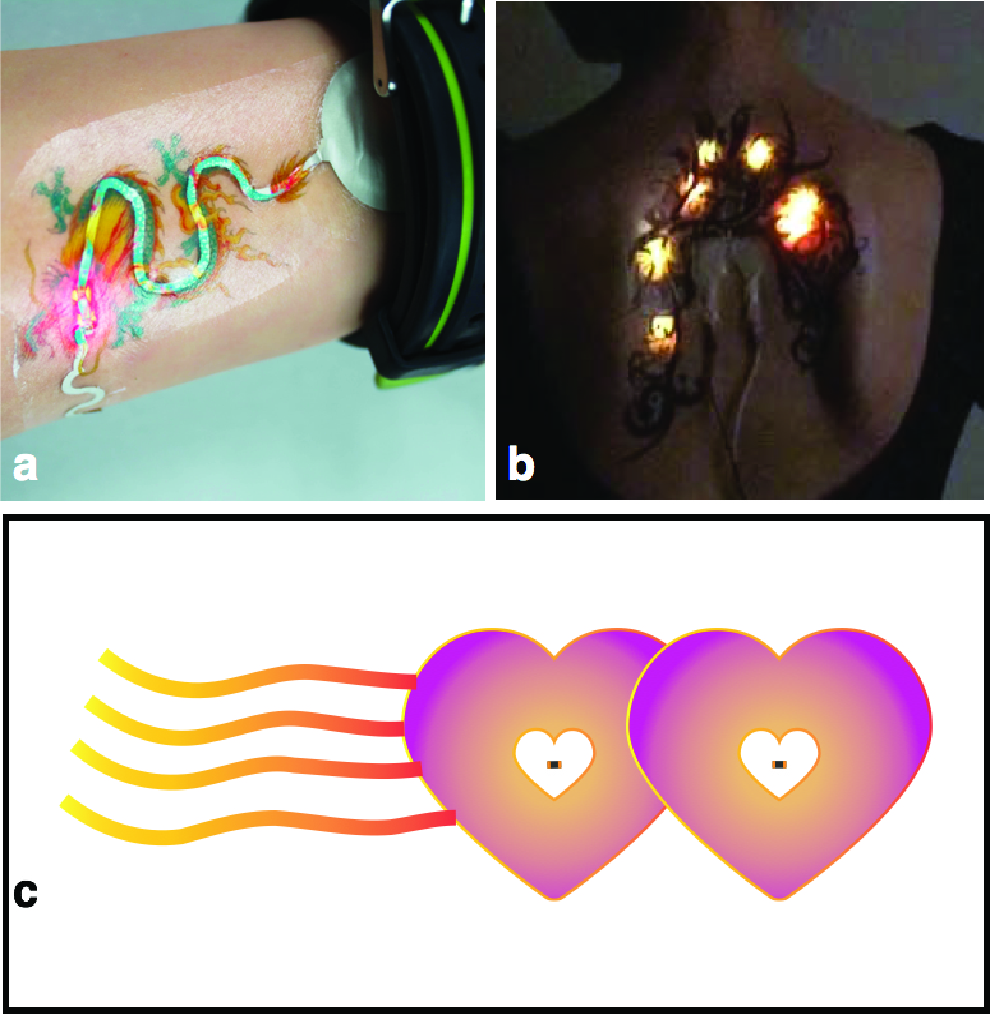
\includegraphics[width=0.8\columnwidth]{figures/Figure5}
\caption{Example of visual design of a Skintillate device. a) A dark colored pattern is printed on the art layer to completely cover the conductive layer, b) A lighter gradient color is printed on the art layer to allow the shape and silver color of the conductive layer to peek through, c) The pattern of the conductive layer is designed to complement the blue flower printed on the art layer, d) The silver conductive layer can be designed to be a design element}
\vspace{-8pt}
\label{fig:design}
\end{figure}
\section{Designing the Visual Aesthetics of Skintillates}
The visual appearance of Skintillates can be designed using both the inkjet printable art layer and the conductive layer. Figure \ref{fig:design} shows a few examples of visual design possibilities. The color and shape of the art layer, which lies on top of the conductive layer when the tattoo is put on skin, can be used to hide or complement the conductive layer. A darker color printed on the art layer that completely overlaps the conductive layer can hide the conductive layer (Fig.\ref{fig:design}a). A lighter color printed on the art layer or a shape that does not completely overlap with the conductive layer allows the silver layer to peek through(Fig.\ref{fig:design}b). The shape of the functional silver conductive layer can also used to enhance the art layer by serving as a subtle decoration or a visual element in the design (Fig.\ref{fig:design}c-d). 



\section{Applications}
We envision a wide range of applications enabled by Skintillates and detail the technical designs and novel interactions across a set of examples in this section.
\subsection{On-Skin Display}
\begin{figure}[!b]
\centering
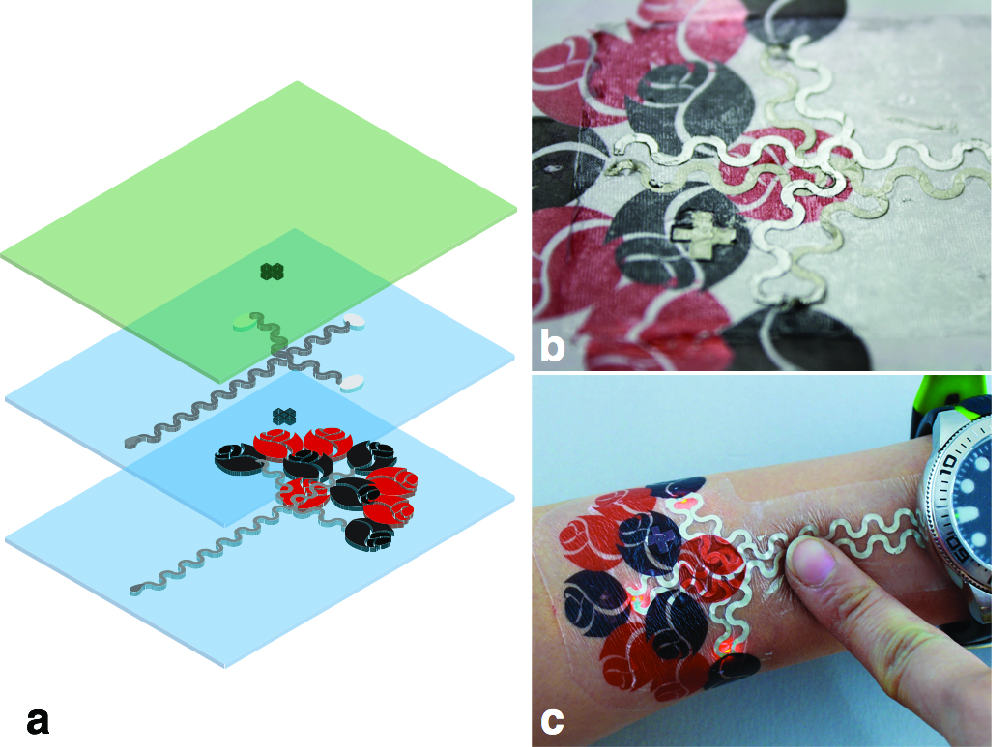
\includegraphics[width=1\columnwidth]{figures/Figure6}
\caption{Example of Skintillates tattoo displays. a) a dragon Skintillates display is powered by the watch and could serve as a point-light display, b) a back Skintillates tattoo that flashes with the beat of the music around the wearer, c) a private Skintillates tattoo flashing according to ECG signals, d) a Skintillates tattoo without a printed art layer decorates an existing permanent tattoo}
\vspace{-8pt}
\label{fig:displays}
\end{figure}
One of the most important aspects of wearing tattoos, either temporary or permanent, is to express personal identity. Skintillates aims to augment the self-expression of tattoo artwork with electronics. In Figure \ref{fig:displays}, we show a few examples of public and private decorative Skintillate displays. Figure \ref{fig:displays}a shows a Skintillate dragon tattoo with red LED eyes that is electrically connected to the watch, and could potentially serve as a point-light display for a smart watch. Figure \ref{fig:displays}b demonstrates a back tattoo with LEDs that flash with the beat of music, which is controlled by an Arduino hidden under the wearer's clothing.  In this example, we also explored the aesthetic of electrical traces and power pads on the tattoo. The power pads, which are traditionally circular or square in shape in printed circuit boards, are designed to look like wings to fit with the aesthetic of the art layer of the tattoo. In Figure \ref{fig:displays}c, we investigated the potential of using Skintillates as a private wearable display for intimate bio-data. We downloaded two sets of publically available test electrocardiogram (ECG) signals from PhysioNet to simulate the heartbeats from two people. In real-life applications, the Skintillates bio-data display can interface with biomonitoring data from commercially available wearable devices. The LEDs are programmed to blink as the signal strength reaches a certain amplitude, mimicking two heartbeats. The user wore the Skintillate ECG display under a shirt so that he/she can lift and glance at the private display or choose to expose it publicly when desired. In Figure \ref{fig:displays}d, we explored the possibility of incorporating a Skintillates display with an existing permanent tattoo. We omitted the art layer in this device and traced one of the tree branches on the silver ink conductive layer to power three LED’s to light up the tattoo flowers.
\subsection{Multi-layer Display}
\begin{figure}
\centering
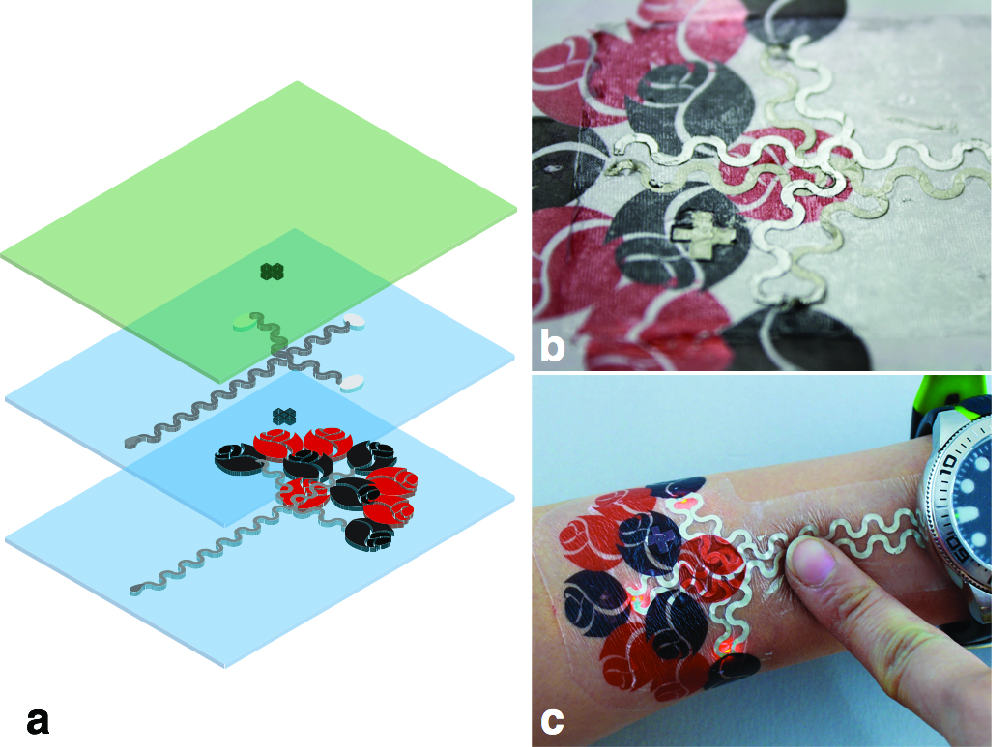
\includegraphics[width=1\columnwidth]{figures/Figure7}
\caption{Multilayer Skintillates Display. a) An exploded illustration of the different layers: a bottom layer consists of the basic Skintillates art and conductive layer, while a second conductive layer is connected to the first layer through vias and the adhesive layer. b) a photograph of the two overlaying but insulated conductive layers, c) the multilayer display under operation while being compressed, showing that it maintains functionality while being flexed.}
\vspace{-8pt}
\label{fig:multilayer}
\end{figure}
\begin{figure*}
\centering
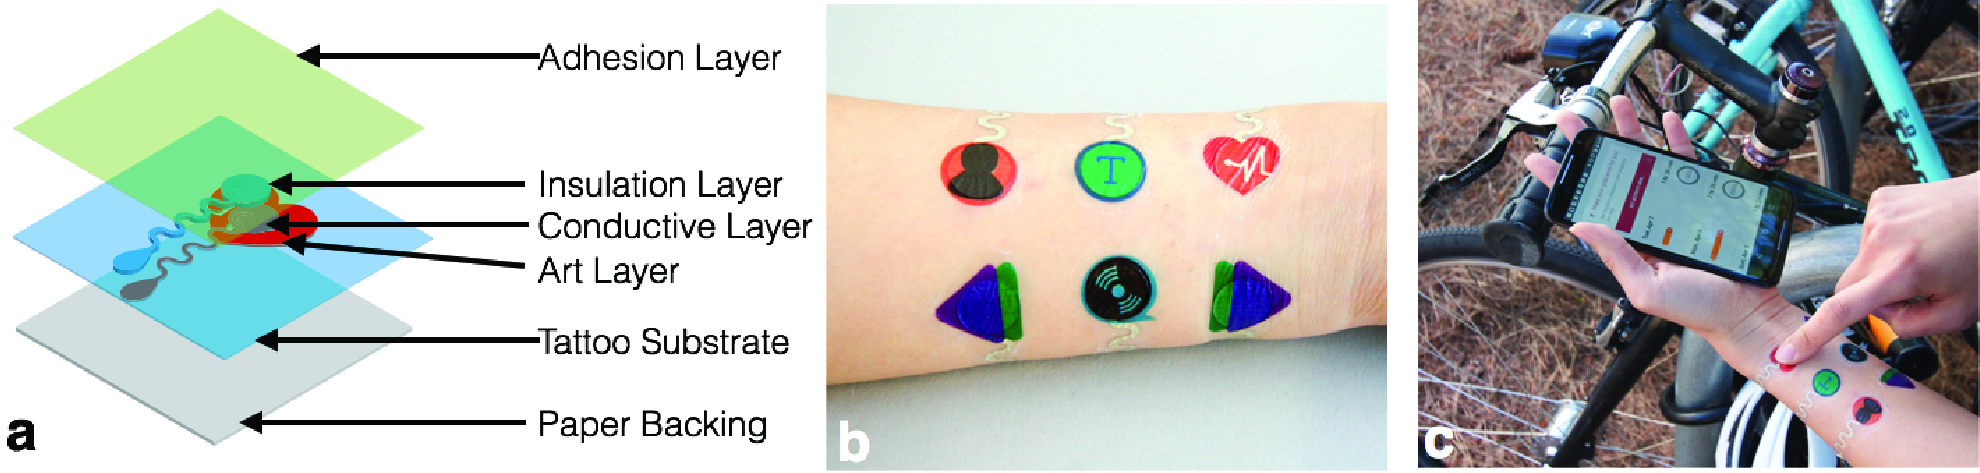
\includegraphics[width=1\textwidth]{figures/Figure8}
\caption{Skintillates Capacitive touch sensing. a) an exploded illustration of a Skintillates capacitive sensor showing one additional insulation layer on top of the conductive layer to prevent charges on skin from interfering with the capacitive touch signal, b) capacitive sensors can be applied on body locations convenient to the wearer; in this case, the inner arm, c) the Skintillates capacitive buttons were used to control a mobile device when the user was active and could not directly access the device screen.}
\vspace{-8pt}
\label{fig:capacitive}
\end{figure*}
Multilayer devices can be fabricated for higher visual or electronic complexity. In printed circuit board design, multiple layers are often needed to achieve desired form and function. Epidermal Electronics have also explored using multilayer devices to support more complicated function\cite{Kim:2014iq}. In arts practices, layers are often used as a means to create depth. In order to fully explore combining arts and electronics on a wearable device, the Skintillates fabrication process should be able to support electrically functional and aesthetically attractive multi-layer devices. Figure \ref{fig:multilayer}a shows an exploded view of a multilayer Skintillates device. In this study, we created a second conductive layer, and the same procedure could be used for creating a second art layer as well. This second conductive layer was screen printed on a separate temporary tattoo substrate, and was released from the paper backing onto the first conductive layer. In order to electrically connect the first and second conductive layers, we created electrical vias, which are openings that allow for electrical connections, by cutting holes in the second layer substrate at appropriate locations. Figure \ref{fig:multilayer}b shows a close-up image of the dual-layer Skintillates device. The top layer traces are insulated from the bottom layer traces with a tattoo layer substrate, and vias are opened at the ends of the traces to allow the LEDs to make contact with both layers of the traces. Although the multilayer Skintillates devices are thicker than the single layer devices, they remain reasonably flexible on skin. In figure\ref{fig:multilayer}c, we show that the dual-layer Skintillates device remains operational even when the traces are being compressed into the skin. 
\subsection{Capacitive Sensing}
Advanced sensing, including capacitive sensing, using epidermal devices is well-established\cite{Jeong:2013km,Frutiger:2015fm,Mannsfeld:2010is}. In many research studies, various algorithms, data processing methods, and grounding schemes are utilized to overcome any technical difficulties usually associated with wearable sensing \cite{Jeong:2013km}.  Through careful material selection, we can achieve sensitivity suitable for common interactive applications. The silver screen printing ink used for Skintillates is very conductive (0.5$\Omega/\square$). 
 This high conductivity is important in capacitor design, where increasing conductivity of the material increases the availability of charge, which directly affects the sensitivity of the capacitive button (Gauss’s Law=$\frac{\sigma}{\epsilon}$).

Capacitive sensing is ubiquitous in interaction design - from sensing nearby gestures to sensing direct touch, the change in electric field carries rich information about the space around us. Skintillates can utilize this sensing mechanism to easily incorporate human interfaces that can be used as local input or as remote signals to control a mobile smartphone.

To ensure reliable performance of the capacitive sensor, both the electronic filtering and the physical device insulation have to be carefully designed. To reduce cost and simplify the design, the raw data of the capacitive sensor is processed and filtered by a commercially available breakout board\footnotemark[1]. To insulate the capacitive sensor against the skin where it is attached, we modify the fabrication steps slightly by adding insulative temporary tattoo substrates without any silver conductive ink on top of the conductive electrodes. This insulative layer prevents electric charges on the surface of the skin from interfering with the desired capacitive touch signal (Fig.\ref{fig:capacitive}a). 

In this study, we demonstrated using capacitive Skintillates buttons to control various mobile smartphone applications (i.e. music, social media, etc) through a low power wireless Bluetooth module\footnotemark[2]. By placing the Skintillates on the inside of the user’s arm (Fig.\ref{fig:capacitive}b), he/she can control the mobile applications on an easily accessible body location (Fig.\ref{fig:capacitive}c). The size and shape of the Skintillates buttons are highly customizable, enabling visual design freedom, such as creating buttons with shapes that represent the application being controlled. Skintillates capacitive sensors are also versatile in that they can be used  as capacitive sliders and wheels in addition to simple buttons.
%Note from Jeff: You claim they can be used as sliders and wheels, but I don't see any justification for this in your paper.  Can you please elaborate or remove?

\footnotetext[1]{Adafruit Capacitive Touch Sensor Breakout MPR121 connected to an Arduino Uno}
\footnotetext[2]{A low-power BLE module provided connectivity to the phone.}

\subsection {On-Skin Resistive Sensor}
\begin{figure} [h!]
\centering
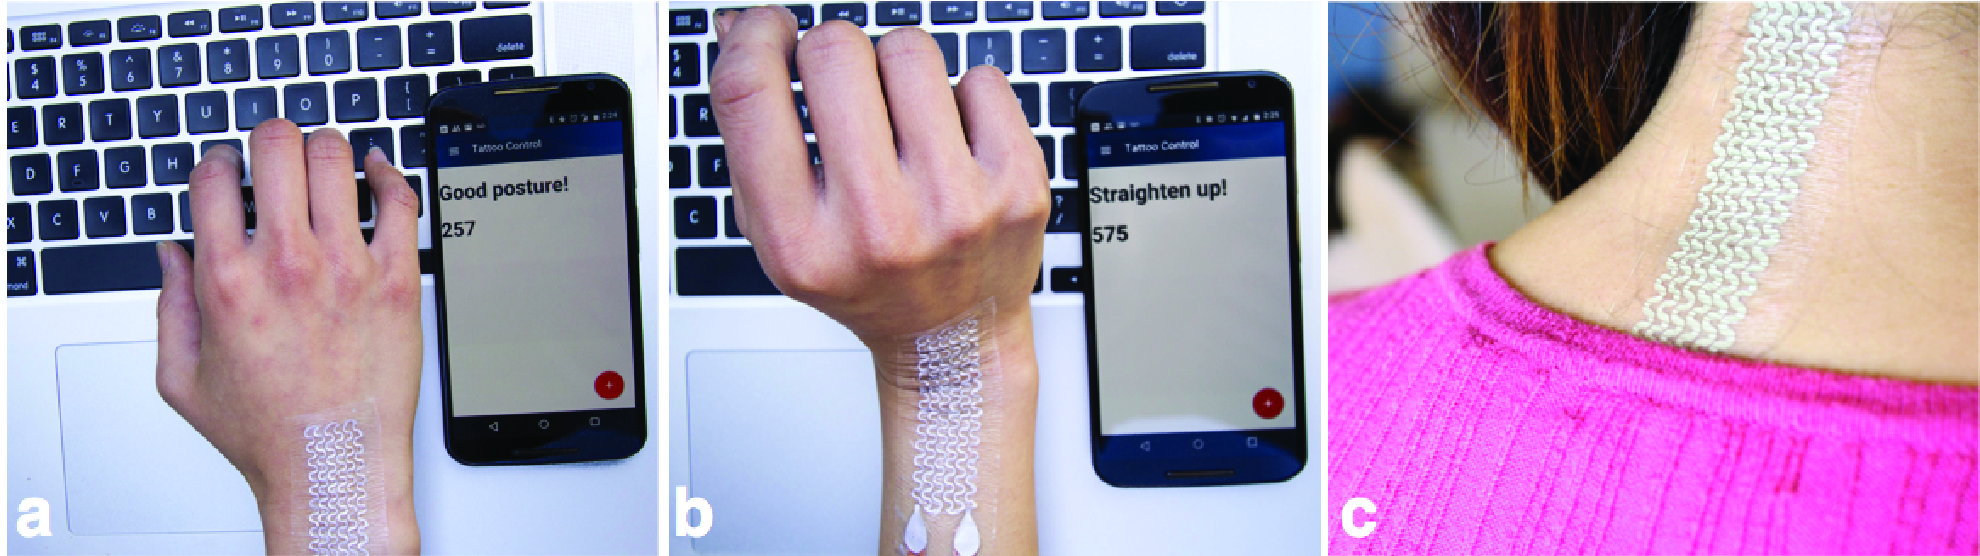
\includegraphics[width=1\columnwidth]{figures/Figure9}
\caption{Skintillates Resistive Sensor. a) Two Skintillates resistive sensors shaped as kites are applied on user's arm. b) the Skintillates sensors are connected to the MakeyMakey to allow the user to control the kites within the computer game.}
\vspace{-8pt}
\label{fig:resisitve}
\end{figure}
Using the human body as a conductor to form a closed circuit to turn on a light is common science experiment, and this sensing method can also enable interesting interactions - such as turning bananas into switches as made popular by the MakeyMakey. We demonstrated that Skintillates can be used as a resistor sensor that is compatible with MakeyMakey. The construction of the Skintillates resistor sensor is very similar to that of the capacitive sensor, with an insulative layer beneath the electrode to prevent electrically connection between the sensor and the skin that it is adhered to. As was the case for the capacitive sensor, the conductivity of the trace material is very important in switch design, where the touched surface needs to be conductive enough to close the switch, so the silver ink is well-suited for this use. Figure \ref{fig:resisitve}a shows two Skintillates resistive sensors shaped as kites, which are connected to the MakeyMakey to act as the left and right arrow of a computer keyboard. The custom buttons are then used as a controller to play a computer game of moving the kite up and down to avoid hitting objects in the sky (Fig.\ref{fig:resisitve}b). A large open-source library and community support are available for prototyping with MakeyMakey, and the Skintillates resistive sensor can be used to enable a wide range of wearable interactions with this platform. 
\subsection {Strain Gauge}
\begin{figure*}
\centering
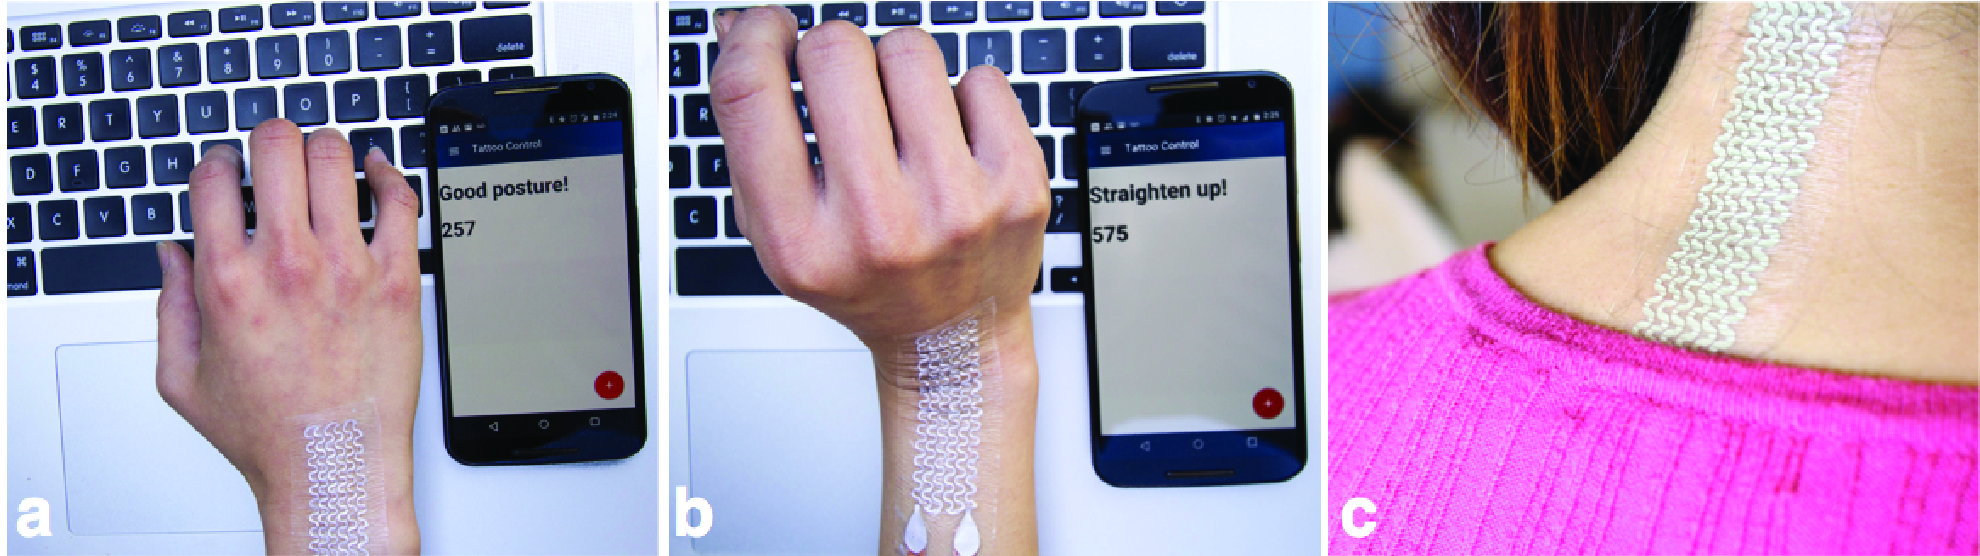
\includegraphics[width=1.0\textwidth]{figures/Figure10}
\caption{Strain gauge for body position sensing. a) The strain gauge reading indicates that the user's wrist is in a correct typing position. b) The strain gauge reading indicates that the user's wrist is not at a correct posture, which causes the mobile phone to send a warning message. c) The strain gauge can also be worn on other body positions, such as the neck and back, to detect movement and posture.}
\vspace{-8pt}
\label{fig:straingauge}
\end{figure*}
The subtle analog motions of the human body carry information that goes beyond that of digital on/off button. The Skintillates strain gauge captures the fluid motion of the human body by translating the movement into a variable resistance. 
 The strain gauge has a longer length in the direction of the wrist bending during typing. As the sensor stretches and contracts with the wrist flexure, the resistance increases and decreases. The change in resistance is detected through a Wheatstone Bridge and amplified using an INA125P operational amplifier. Before amplification, the variation in the resistance ranges from 37$\Omega$ (when wrist is flat) to 54$\Omega$ (full wrist flexure). The amplified analog value is read using an Arduino Uno and transmitted to a mobile phone via Bluetooth, where the value is then displayed on the screen of the mobile phone. Appropriate warning messages are displayed as the user’s wrist posture changes. Although the strain gauge is located on the wrist in this example, this device can also be used for back posture by placing the sensor on the neck (Fig.\ref{fig:straingauge}c). In addition to posture detection, Skintillates strain gauges can serve as an always-available, non-intrusive sensor to detect different gestures for electronic interactions or be incorporated into performance art. 

\section {User Study}
\begin{figure} [b!]
\centering
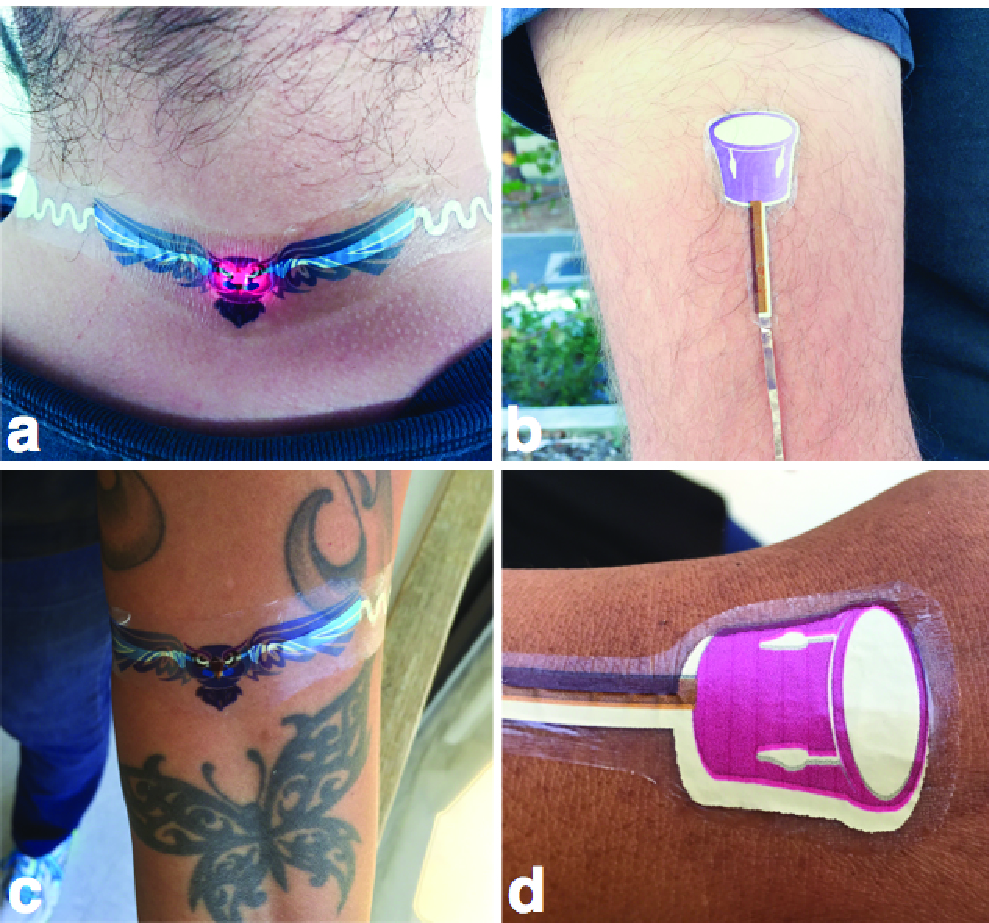
\includegraphics[width=1\columnwidth]{figures/Figure11}
\caption{Representative Pictures of Skintillates Devices in User Study. Participants were free to apply the Skintillate tattoo on any body location, example applied body locations include a) neck, and b) arm. c) Skintillate LED displays used in the study utilize small 0603 LED parts, which allows the Skintillate tattoo to retain its conformal profile. d) Skintillates resistive sensor used in the study worn on arm. }
\vspace{-8pt}
\label{fig:userstudy}
\end{figure}
While the functionality and signal quality of Skintillates is an important part of detailing its design, we were interested in how Skintillates would perform under everyday, natural conditions with real users.  We were also interested in users’ degree of comfort and reactions to the Skintillates aesthetics.  To improve our understating of these issues we conducted a series of user studies.
\subsection {Study Participants}
We recruited 10 participants (6 male and 4 female) through an office mailing list to be interviewed and wear a pre-designed Skintillates device.  Our participants ranged in age from 25 to 42 years old with 29.7 being the mean.  
\subsection {Procedure}
Each participant arrived and was met individually during the start of the workday.  Three previously designed and fabricated Skintillates was presented to them along with an overview of the project and description of the individual elements of the Skintillates device.  The three Skintillates that were chosen in the study represented a broad range of sensing and display types: (1) a Skintillates display measuring 6.5 in x 1.0 in and connected to 3.3V coin cell batteries (Fig.\ref{fig:userstudy}a,c), (2) a Skintillates resistive sensor measuring 1.3 in x 0.8 in and connected to a MakeyMakey (Fig.\ref{fig:userstudy}b,d), and (3) two unaltered temporary tattoos without any conductive layer to be used as a control. Participants were invited to select a location to wear each Skintillates for the duration of a workday (ranging from 8-10 hours), and we applied the devices on their chosen locations. 

Simple functionality tests, such as turning on the LED’s on the Skintillates display and controlling computer keys with the Skintillates resistive sensor, were performed immediately after the devices were applied on skin to confirm functionality. The Skintillates displays were continuously powered and participants were asked to contact the researcher if the devices were to stop functioning. After the Skintillates devices were applied and tested, the participants were asked to resume their normal daily work activities wearing the devices and to return at a predetermined time at the end of the workday. The work functions participants performed included office activities such as typing, writing, and manipulating light machinery (i.e. 3D printers and thermal oven).

At the end of the work day, participants returned and were interviewed about their qualitative experience of wearing Skintillates.  We also conducted a survey to  quantitatively measure comfort levels.   Finally, the same  functionality tests performed in the beginning of the study were performed on the Skintillates devices to assess their durability. Participants were free to choose whether they would remove or continue to wear the Skintillates devices at the end of the interview.    In both conditions, participants completed a follow-up survey the following day about the social aspects of Skintillates.
\subsection {Discussion and Findings}
All ten participants chose to attach all of the Skintillates and control tattoos and completed the study. ****need to add a bit more here***.  We analyzed our interview data using a thematic analysis to reveal patterns across data sets associated our research. These themes are discussed in the subsections that follow.
\subsubsection{Body Location Choices}
The majority of the users chose to put the Skintillates devices on their arms, while one user placed the Skintillates display on the back of the neck. When asked about their decision of the placement of the Skintillates devices, users cited the shape of the Skintillates devices and their outfit of the day to be the main reason for their choice. All of the Skintillates displays were worn in a publically visible locations - uncovered by the participants’ clothing. The wearing location of the Skintillates resistive sensors were based on participants’ preference on on-skin keyboard interactions. For example, R2 chose to put the resistive sensors on the inside of his/her forearm because that user preferred using his/her thumb to control the on-skin keyboard while resting their palm on their arm. 
\subsubsection{Comfort and Social Acceptably}
Participants were asked at the end of the 8-10 hour wearing period to rate the comfort of the Skintillates display on a 1-10 scale (with 10 being most comfortable).  Users made this assessment with and without consideration of the battery connection (i.e. the copper tape connected to the battery). Since different body locations contain different nerve endings and degrees of sensitivity, it is difficult to generalize the results.  However, we believe the quantitative results were valuable since they provide insights on the perceived comfort for the user-selected wearing locations. 
The average comfort of the control temporary tattoo was 9.2 (SD = 0.42). Without considering the battery connection, the comfort of the Skintillates display and resistive sensor was 8.2 (SD=0.67) and 8.8 (SD = 0.35) respectively. Most participants described Skintillates devices as something that they \textit{“don’t even feel after a while”}and \textit{“feels very similar to a normal temporary tattoo”}, and the small 0.5mm-thick 0603 electronic LEDs were described as \textit{“little bumps”} and did not appear to significantly affect any of the participants' comfort assessment.  None of the participants mentioned the electronic parts as an undesirable element of the design in terms of comfort.
Not surprisingly, when considering the battery connection, the comfort level of the display decreased to 7.1 (SD = 0.53). Participants were most bothered by the battery connections and the hard coin cell batteries. 

A exciting result was that even at the end of the formal wearable portion of the study, 8 of the 10 participants chose to continue wearing both Skintillates devices.  In the follow-up survey the next day, participants were asked how long and why they continued to wear their Skintillates devices even after they were invited to remove them. All of the participants who had plans to interact with friends and family after the work day (8 out of 10) kept wearing the tattoo after the study so that they could show the Skintillates devices to their loved ones - “I wanted to keep it because I thought my kids would think that this is the coolest thing ever”. Two of the participates mentioned that although they did not have prior plans to go out after work that night, they each independently decided to go to a public place (one to a restaurant for take-out, and one to a sports bar) to show off the Skintillates display. R7, who went to a sports bar to show off the tattoo, commented that \textit{“it seems to be a waste not to show this to someone”}. Although all of the participants took off the Skintillates devices before showering or going to bed, all of them said that they took the devices off very carefully as to not damage them so that they could reuse them in the future. 

Even more encouraging, all of our participants reported that they would like to wear the Skintillates device again, and expressed a desire to design their own Skintillates displays and sensors. 

\subsubsection{Durability}
During the study only one of the ten Skintillates displays was damaged. In the affected devices, the battery wire of the device was caught on the chair and was torn when the user stood up after wearing the device for approximately five hours. All the remaining nine displays functioned perfectly throughout the entire study. Within our lab group, we have found that Skintillates devices can remain functional for days after multiple removal and reapplication steps. We hope to perform a longer-term user study in the future to examine the limit of the durability of the different types of Skintillates devices. 
\subsubsection{Envisioned Applications}
We asked participants after wearing Skintillates for the 8-10 hour day to describe imagined scenarios of usage with such devices. One class of applications were around creative interactions with nearby devices – ``\textit{a henna tattoo that can control everything in my house”}'', ``\textit{“tattoo buttons that make people massage my back when they need to turn on the light”}'', or to ``\textit{“control things with a Spiderman gesture”}''.  Another theme was more specific usage as a decorative body display – ``\textit{“put some evil red eyes on my [permanent] skull tattoo”}'', ``\textit{“burning man costume”}'',  ``\textit{a car tattoo with cycling LED’s on the wheels}''. We also found deep reflection on more functional designs -- such as a ``\textit{“turning signal for motorcyclists [mounted on the back of the neck]}'' or ``\textit{a red/green light [to indicate if] I want to be bothered by people)}''.
*** Need some 2-3 sentences to wrap up user study section…***
\section {Limitations}
While we have a highlighted a number of benefits of the Skintillates design, there are several important limitations to note of the current technology. First, while the Skintillates device and its electrical traces are highly flexible, the external electrical interconnects to batteries for power are not.  These are currently made with copper tape which does not have the same elastic properties as the Skintillates. This difference in material properties not only causes that electrical connection to be the mechanically weakest point of the device but also was a source of discomfort in our users. We believe this problem can be overcome by stabilizing the connection using a small piece of medical-grade tape - the tape relieves most of the stress exerted on the connection and prevents tearing of the connection. In future work, we would like to develop a flexible electrical connector that can move with the skin and provide an electrical interface with the Skintillates device.

Another limitation lies in the reusability of the Skintillates devices. In the research team's experience, the Skintilltaes devices can be reused at least four to five times if the devices contains finely traced (\textless 2mm) circuits and many more times if the for sensors consist of only large conductive patches. The reusability of the devices could potentially be improved with a thin (\textless10\SI{}{\micro\metre})
%Make um into units
 spray-on encapsulating layer. Further studies can also be performed to optimize the electronic design for durability. 

\section {Discussion and future applications}
The development of Skintillates has significant impact in customizable flexible and wearable electronics and their applications. The simple fabrication process of Skintillates provides an alternative to prototyping with polymer casting and curing.  The design freedom, in terms of electrical, functionality, and visual aesthetic design, of Skintillates can support a diverse ecosystem of users from diverse backgrounds, including engineers, designers, and artists. We plan to continue to investigate the creation of more complex interactive electronics on Skintillates devices and studying how these devices can blend artfully and seamlessly into people's daily lives. 

In order to support more complex interactions, we would like to develop flexible electronics to replace the Arduino and MakeyMakey that the Skintillates are currently interfacing with. By using thin substrate and conductive polymeric electrical traces, we hope to create a multipurpose open-source development board specific for flexible wearable applications. 

We would also like to expand upon the current aesthetic design of Skintillates by collaborating with artists, in particular tattoo artists and performance artists, to create  novel responsive and interactive Skintillates designs. Since Skintillates sensors and programmable displays can be adhered on a diverse suite of body locations, we would like to explore some creative interaction and data display methods that are tailored to the human body instead of an electronic screen. 

\section {conclusion}
In this paper we presented a novel wearable on-skin technology - Skintillates.  We demonstrated its wide range of capabilities from capacitive and resistive sensing input to point-light output, which are augmented with an easily inkjet-printable customizable full-color aesthetic design.  We presented a range of functional designs across a set of application domains such as health and well-being, mobile device interaction, social connectedness, and personal fashion and lifestyle. We investigated both in the lab and in the field via a user study how its thin (typically approximately 36\SI{}{\micro\metre}) and flexible material design easily conforms to the skin making it comfortable to wear for an extended period of time. We also measured its durability over time with a wide range of users, demonstrating how Skintillates performs well during everyday activities - remaining functional for hours or even days. Finally, we highlighted how our use of common design software, low-cost materials, and simplified fabrication techniques make Skintillates a truly accessible technology.  We hope that this functional, comfortable, and accessible on-skin device will be enthusiastically adopted by a diverse suite of practitioners and inspire a range of novel applications and aesthetic designs for our future wearables.





%\section{Acknowledgments}

%We thank CHI, PDC and CSCW volunteers, and all publications support
%and staff, who wrote and provided helpful comments on previous
%versions of this document.  Some of the references cited in this paper
%are included for illustrative purposes only.  \textbf{Don't forget
%to acknowledge funding sources as well}, so you don't wind up
%having to correct it later.

% Balancing columns in a ref list is a bit of a pain because you
% either use a hack like flushend or balance, or manually insert
% a column break.  http://www.tex.ac.uk/cgi-bin/texfaq2html?label=balance
% multicols doesn't work because we're already in two-column mode,
% and flushend isn't awesome, so I choose balance.  See this
% for more info: http://cs.brown.edu/system/software/latex/doc/balance.pdf
%
% Note that in a perfect world balance wants to be in the first
% column of the last page.
%
% If balance doesn't work for you, you can remove that and
% hard-code a column break into the bbl file right before you
% submit:
%
% http://stackoverflow.com/questions/2149854/how-to-manually-equalize-columns-
% in-an-ieee-paper-if-using-bibtex
%
% Or, just remove \balance and give up on balancing the last page.
%
\balance

\bibliographystyle{acm-sigchi}
\bibliography{skintillates}
\end{document}
